\documentclass[]{abntex2}
\usepackage{lmodern}			% Usa a fonte Latin Modern
\usepackage[T1]{fontenc}		% Selecao de codigos de fonte.
\usepackage[utf8]{inputenc}		% Codificacao do documento (acentuação)
\usepackage{indentfirst}		% Indenta o primeiro parágrafo de cada seção.
\usepackage{nomencl} 			% Lista de simbolos
\usepackage{color}				% Controle das cores
\usepackage{graphicx}			% ISnclusão de gráficos
\usepackage{microtype} 			% para melhorias de justificação
\usepackage{amsmath}
\usepackage{float}
% Pacotes adicionais, usados apenas no âmbito do Modelo Canônico do abnteX2
\usepackage{lipsum}				% para geração de dummy text
\usepackage[brazilian,hyperpageref]{backref}% Paginas com as citações na bibl
\usepackage[alf]{abntex2cite}	% Citações padrão ABNT
\usepackage{tcolorbox} % Para criar a caixa


\usepackage{amssymb}
\usepackage{hyperref} 


\usepackage{multirow}
\usepackage[table]{xcolor}
%\usepackage{colortbl}
\usepackage[table]{xcolor}

% ---
% Informações de dados para CAPA e FOLHA DE ROSTO
% ---
\titulo{Lista 1 - Processamento de Imagens}
\autor{Lorran de Araújo Durães Soares\thanks{lorranspbr@gmail.com}}
\data{2024}
% ---

% ---
% Configurações de aparência do PDF final
% alterando o aspecto da cor azul
\definecolor{blue}{RGB}{41,5,195}

% ---
% compila o indice
% ---
\makeindex
% ---

% ---
% Altera as margens padrões
\setlrmarginsandblock{3cm}{3cm}{*}
\setulmarginsandblock{3cm}{3cm}{*}
\checkandfixthelayout
% O tamanho do parágrafo é dado por:
\setlength{\parindent}{1.3cm}
% Controle do espaçamento entre um parágrafo e outro:
\setlength{\parskip}{0.2cm}  % tente também \onelineskip
% Espaçamento simples
\SingleSpacing


\begin{document}

% Retira espaço extra obsoleto entre as frases.
\frenchspacing 

\maketitle

\section*{\textbf{Questão 1}}
\addcontentsline{toc}{section}{Questão 1}

\textit{Vamos considerar o seguinte band-pass filter no domínio de Fourier:}

\begin{equation}
\widehat{H}(\omega) =
\begin{cases}
    1, & -b \leq \omega \leq -a, \\
    1, & a \leq \omega \leq b, \\
    0, & \text{caso contrário.}
\end{cases}
\label{eq:H}
\end{equation}

\textit{Calcule o núcleo do filtro no domínio espacial resolvendo a transformada inversa de Fourier da expressão \ref{eq:H}:}

\begin{equation}
H(x) = \int_{-\infty}^{\infty} \widehat{H}(\omega) \exp(2 \pi j \omega x) \, d\omega,
\label{eq:h}
\end{equation}

\textbf{Resolução:}

Vamos então calcular o filtro no espaço do domínio resolvendo a integral da equação \ref{eq:h}:

\begin{center}
$
H(x) = \int_{-\infty}^{\infty} \widehat{H}(\omega) \exp(2 \pi j \omega x) \, d\omega = 
\int_{-\infty}^{-b} 0 \cdot \exp(2 \pi j \omega x) \, d\omega + \int_{-b}^{-a} 1 \cdot \exp(2 \pi j \omega x) \, d\omega + 
$

$
\int_{-a}^{-a} 0 \cdot \exp(2 \pi j \omega x) \, d\omega + \int_{a}^{b} 1 \cdot \exp(2 \pi j \omega x) \, d\omega + \int_{b}^{\infty} 0 \cdot \exp(2 \pi j \omega x) \, d\omega = 
$

$
\int_{-b}^{-a} \exp(2 \pi j \omega x) \, d\omega + \int_{a}^{b} \exp(2 \pi j \omega x) \, d\omega = \dfrac{1}{2\pi jx}\cdot \exp(2\pi j \omega x)\bigg|_{-b}^{-a} + \dfrac{1}{2\pi jx}\cdot \exp(2\pi j \omega x) \bigg|_{a}^{b} = 
$

$
\dfrac{1}{2\pi jx}\cdot \{ [\exp(-2 \pi j a x)- \exp(-2 \pi j b x)] + [\exp(2 \pi j b x)- \exp(2 \pi j a x)]\} =  
$

$
\dfrac{1}{2\pi jx}\cdot \{ [\cos (2\pi a x) -j \sin (2\pi a x) - (\cos (2\pi b x) - j \sin (2\pi b x)) ] + [\cos (2\pi b x) + j \sin (2\pi b x) - (\cos (2\pi a x) + j \sin (2\pi a x))] \}  =
$

$
\dfrac{1}{2\pi jx}\cdot [\cos (2\pi a x) -j \sin (2\pi a x) - \cos (2\pi b x) + j \sin (2\pi b x) + \cos (2\pi b x) + j \sin (2\pi b x) - \cos (2\pi a x) - j \sin (2\pi a x)] = 
$

$
\dfrac{1}{2\pi jx}\cdot [- 2j \sin (2\pi a x) + 2j \sin (2\pi b x)] = \dfrac{1}{\pi x}\cdot [- \sin (2\pi a x) + \sin (2\pi b x)] 
$

\tcbset{
    colframe=black!75!black,    % Cor da borda
    colback=gray!10!white,     % Cor do fundo
    boxrule=0.5mm,             % Espessura da borda
    arc=2mm,                   % Curvatura dos cantos
    left=0pt,                  % Margem esquerda
    right=0pt,                 % Margem direita
    top=2pt,                   % Margem superior
    bottom=2pt,                % Margem inferior
    boxsep=0pt,                % Espaço entre a borda e o conteúdo
}

\begin{tcolorbox}
\[
	\therefore H(x) = \dfrac{1}{\pi x}\cdot [\sin (2\pi b x) - \sin (2\pi a x)]
\]
\end{tcolorbox}

\end{center}

% ==================================================================================
% ==================================================================================
% ==================================================================================
% ==================================================================================
% ==================================================================================
% ==================================================================================
% ==================================================================================

\section*{\textbf{Questão 2}}
\addcontentsline{toc}{section}{Questão 2}

\textit{Demonstre a seguinte expressão da aula2.pdf:}

\begin{equation}
	x(m, n) = \frac{1}{4\pi^2} \int_{-\pi}^{\pi} \int_{-\pi}^{\pi} X(\omega_1, \omega_2) \exp \left( j (m \omega_1 + n \omega_2) \right) d\omega_1 d\omega_2 \label{eq:x}
\end{equation}

\textbf{Resolução:}

Temos que a transformada de Fourier da sequência $x(m,n)$ é dada por:

\begin{center}
\begin{equation}
	X(\omega_1, \omega_2) = \sum_{m=-\infty}^{+\infty} \sum_{n=-\infty}^{+\infty} x(m, n) \exp \left( -j (m \omega_1 + n \omega_2) \right), \quad -\pi \leq \omega_1, \omega_2 \leq \pi	
	\label{eq:aa}
\end{equation}
	
\end{center}

Vamos então mostrar que vale a expresão \ref{eq:x}. De fato, da equação \ref{eq:aa}, teremos que:

\begin{equation*}
	X(\omega_1, \omega_2) \cdot \exp \left( j (p \omega_1 + q \omega_2) \right)= \sum_{m=-\infty}^{+\infty} \sum_{n=-\infty}^{+\infty} x(m, n) \exp \left( -j (m \omega_1 + n \omega_2) \right) \cdot \exp \left( j (p \omega_1 + q \omega_2) \right) \Leftrightarrow 	
\end{equation*}

\begin{equation*}
	\Leftrightarrow \int_{-\pi}^{\pi} \int_{-\pi}^{\pi}X(\omega_1, \omega_2) \cdot \exp \left( j (p \omega_1 + q \omega_2) \right)d\omega_1 d\omega_2= 
\end{equation*}

\begin{equation}
	\int_{-\pi}^{\pi} \int_{-\pi}^{\pi}\sum_{m=-\infty}^{+\infty} \sum_{n=-\infty}^{+\infty} x(m, n) \exp \left( -j ((m-p) \omega_1 + (n-q) \omega_2) \right) \cdot d\omega_1 d\omega_2
	\label{eq:pre}
\end{equation}

Coniderando o segundo termo da equação \ref{eq:pre}, invertendo a ordem entre integração e somatório, teremos que:

\begin{equation}
	\sum_{m=-\infty}^{+\infty} \sum_{n=-\infty}^{+\infty} x(m, n) \int_{-\pi}^{\pi} \int_{-\pi}^{\pi}\exp \left( -j ((m-p) \omega_1 + (n-q) \omega_2) \right) \cdot d\omega_1 d\omega_2
	\label{eq:pre1}
\end{equation}

Porém, note que:

\begin{itemize}
	\item Se $m=p$ e $n=q$, então:
	
	\begin{equation*}
		\int_{-\pi}^{\pi} \int_{-\pi}^{\pi}\exp \left( -j ((m-p) \omega_1 + (n-q) \omega_2) \right) \cdot d\omega_1 d\omega_2 = \int_{-\pi}^{\pi} \int_{-\pi}^{\pi}\exp (0) \cdot d\omega_1 d\omega_2 =
	\end{equation*}
	
	\begin{equation*}
		\int_{-\pi}^{\pi} \int_{-\pi}^{\pi} d\omega_1 d\omega_2 = \int_{-\pi}^{\pi} \omega_1 \bigg|_{-\pi}^{\pi} d\omega_2 = 2\pi \cdot \omega_2 \bigg|_{-\pi}^{\pi} = 2\pi \cdot 2\pi = 4\pi^{2}	
	\end{equation*}

	\item Se $m=p$ ou $n=q$, supondo, sem perca de generalidade, que $m=p$ e $n \neq  q$, teremos então que:
	
	\begin{equation*}
		\int_{-\pi}^{\pi} \int_{-\pi}^{\pi}\exp \left( -j ((m-p) \omega_1 + (n-q) \omega_2) \right) \cdot d\omega_1 d\omega_2 = \int_{-\pi}^{\pi} \int_{-\pi}^{\pi}\exp \left( -j ((n-q) \omega_2) \right) \cdot d\omega_1 d\omega_2 =
	\end{equation*}
	
	\begin{equation*}
		\int_{-\pi}^{\pi} \exp \left( -j ((n-q) \omega_2) \right) \cdot \int_{-\pi}^{\pi} d\omega_1 d\omega_2 = 2\pi \cdot \int_{-\pi}^{\pi} \exp \left( -j ((n-q) \omega_2) \right) \cdot d\omega_2 = 
	\end{equation*}

	\begin{equation*}
		\dfrac{2\pi}{-j (n-q)}\cdot \exp \left( -j ((n-q) \omega_2) \right) \bigg|_{-\pi}^{\pi} = \dfrac{2\pi}{-j (n-q)}\cdot [\exp \left( -j ((n-q) \pi) \right) - \exp \left( j ((n-q) \pi) \right)] = 
	\end{equation*}

	\begin{equation*}
		\dfrac{2\pi}{-j (n-q)}\cdot [\cos((n-q) \pi - j\sin ((n-q) \pi)) - \cos((n-q) \pi - j\sin ((n-q) \pi)) ] = 
	\end{equation*}

	\begin{equation*}
		\dfrac{2\pi}{-j (n-q)}\cdot [- 2j\sin ((n-q) \pi)]
	\end{equation*}

	Mas, $(n-q)\in Z$, logo $\sin((n-q)\pi) = 0$. Então: 

	\begin{equation*}
		\dfrac{2\pi}{-j (n-q)}\cdot [- 2j\sin ((n-q) \pi)] = 0 
	\end{equation*}

	\item Se $m \neq p$ e $n\neq q$, teremos então que:
	
	\begin{equation*}
		\int_{-\pi}^{\pi} \int_{-\pi}^{\pi}\exp \left( -j ((m-p) \omega_1 + (n-q) \omega_2) \right) \cdot d\omega_1 d\omega_2 = 
	\end{equation*}

	\begin{equation*}
		\dfrac{1}{-j(m-p)} \int_{-\pi}^{\pi} [\exp \left( -j ((m-p) \pi + (n-q) \omega_2) \right) - \exp \left( -j (-(m-p)\pi + (n-q) \omega_2) \right) ]d\omega_2 = 
	\end{equation*}
	
	\begin{equation*}
		\dfrac{1}{-(m-p)(n-q)} [\exp \left( -j ((m-p) \pi + (n-q) \pi) \right) - \exp \left( -j ((m-p) \pi - (n-q) \pi) \right) -  
	\end{equation*}

	\begin{equation*}
		\exp \left( -j (-(m-p)\pi + (n-q) \pi) \right) + \exp \left( -j (-(m-p)\pi - (n-q) \pi) \right)] 
	\end{equation*}

	Novamente, como $\sin(x\pi) = 0$ para qualquer $x$ inteiro, então sobrarão apenas os cossenos. Assim:

	\begin{equation*}
		\dfrac{1}{-(m-p)(n-q)} [\cos \left((m-p) \pi + (n-q) \pi \right) - \cos \left((m-p) \pi - (n-q) \pi \right) -
	\end{equation*}
	
	\begin{equation*}
		\cos \left(-(m-p)\pi + (n-q) \pi \right) + \cos \left(-(m-p)\pi - (n-q) \pi \right)] 
	\end{equation*}

	Chamando $m-p = x$ e $n-q=y$, teremos que:

	\begin{equation*}
		\dfrac{1}{-xy} [\cos \left(x \pi + y \pi \right) - \cos \left(x \pi - y \pi \right) - \cos \left(-x\pi + y \pi \right) + \cos \left(-x\pi - y \pi \right)] 
	\end{equation*}

	Como $\cos (x) = \cos (-x)$, resultará também, que:

	\begin{equation*}
		\dfrac{1}{-xy} [2\cos \left(x \pi + y \pi \right) - 2\cos \left(x \pi - y \pi \right)] = \dfrac{1}{-xy} [2\cos \left(\pi(x + y) \right) - 2\cos \left(\pi(x - y) \right)] 
	\end{equation*}

	Porém, note que:

	\begin{itemize}
		\item Se $x + y$ é par, então $x$ e $y$ são pares ou $x$ e $y$ são ímpares, o que implicaria que $x-y$ é par.
		\item Se $x + y$ é impar, então ou $x$ ou $y$ é impar, o que implicaria que $x-y$ é ímpar.
	\end{itemize}

	Logo, para o primeiro caso:

	\begin{equation*}
		\dfrac{1}{-xy} [2\cos \left(\pi(x + y) \right) - 2\cos \left(\pi(x - y) \right)] = \dfrac{1}{-xy} (2-2) = 0. 
	\end{equation*}

	Para o segundo caso:

	\begin{equation*}
		\dfrac{1}{-xy} [2\cos \left(\pi(x + y) \right) - 2\cos \left(\pi(x - y) \right)] = \dfrac{1}{-xy} (-2-(-2)) = 0. 
	\end{equation*}

	Ou seja:

	\begin{equation*}
		\int_{-\pi}^{\pi} \int_{-\pi}^{\pi}\exp \left( -j ((m-p) \omega_1 + (n-q) \omega_2) \right) \cdot d\omega_1 d\omega_2 = 0
	\end{equation*}

\end{itemize}

Logo, a integral da expressão \ref{eq:pre1} só tem resultado diferente de 0 se $m=p$ e $n=q$. Logo, a equação \ref{eq:pre1} resultará em:

\begin{equation*}
	\sum_{m=-\infty}^{+\infty} \sum_{n=-\infty}^{+\infty} x(m, n) \int_{-\pi}^{\pi} \int_{-\pi}^{\pi}\exp \left( -j ((m-p) \omega_1 + (n-q) \omega_2) \right) \cdot d\omega_1 d\omega_2 = 4\pi^{2}\cdot x(p,q)
\end{equation*}

Substituindo então na equação \ref{eq:pre}, teremos então que:

\begin{equation*}
	\int_{-\pi}^{\pi} \int_{-\pi}^{\pi}X(\omega_1, \omega_2) \cdot \exp \left( j (p \omega_1 + q \omega_2) \right)d\omega_1 d\omega_2 = 4\pi^{2}\cdot x(p,q)
\end{equation*}

\begin{tcolorbox}
	\[
		\therefore x(p, q) = \frac{1}{4\pi^2} \int_{-\pi}^{\pi} \int_{-\pi}^{\pi} X(\omega_1, \omega_2) \exp \left( j (p \omega_1 + q \omega_2) \right) d\omega_1 d\omega_2
	\]
	\end{tcolorbox}

% ==================================================================================
% ==================================================================================
% ==================================================================================
% ==================================================================================
% ==================================================================================
% ==================================================================================
% ==================================================================================

\section*{\textbf{Questão 3}}
\addcontentsline{toc}{section}{Questão 3}

\textit{Sejam duas matrizes não singulares $A,B \in R^{N \times N}$. Mostre que o produto de Kronecker satisfaz:}

\begin{equation}
	{(A \otimes B)}^{-1} = A^{-1} \otimes B^{-1}
	\label{eq:inv}
\end{equation}

\textbf{Resolução:}

Vamos primeiramente provar que vale a seguinte propriedade, onde $A,B,C,D \in R^{N \times N}$:

\begin{equation*}
	(A \otimes B)(C \otimes D) = (AC \otimes BD)
\end{equation*}

De fato, utilizando a multiplicação entre blocos de matrizes, teremos que:

\begin{equation*}
	{[(A \otimes B)(C \otimes D)]}_{ij} = [a_{i1}B \cdots a_{iN}B][c_{1j}D \cdots c_{Nj}D]^{T} = \sum_{k=1}^{N} (a_{ik}B)(c_{kj}D) = 
\end{equation*}

\begin{equation*}
	\sum_{k=1}^{N} a_{ik}c_{kj}BD = {[AC]}_{ij} BD =  {[(AC) \otimes (BD)]}_{ij}
\end{equation*}

para quaisquer $i,j \in \{1,..,N\}$. Logo, podemos concluir que vale:

\begin{equation*}
	(A \otimes B)(C \otimes D) = (AC \otimes BD)
\end{equation*}

Logo, fazendo o uso da propriedade demonstrada acima, iremos provar então a equação \ref{eq:inv}. 

Por hipótese, $A$ e $B$ são não singulares, então temos que existe as matrizes inversas $A^{-1}$ e $B^{-1}$. Queremos mostrar então que:

\begin{equation*}
	(A \otimes B)(A^{-1} \otimes B^{-1}) = I_{N^2}
\end{equation*}
e
\begin{equation*}
	(A^{-1} \otimes B^{-1}) (A \otimes B) = I_{N^2}
\end{equation*}

De fato:

\begin{equation*}
	(A \otimes B)(A^{-1} \otimes B^{-1}) = (A{A}^{-1} \otimes B{B}^{-1}) = I_N \otimes I_N = I_{N^2}
\end{equation*}

e

\begin{equation*}
	(A^{-1} \otimes B^{-1}) (A \otimes B) = ({A}^{-1}A \otimes {B}^{-1}B) = I_N \otimes I_N = I_{N^2}
\end{equation*}

Portanto, podemos concluir que:

\begin{tcolorbox}
	\[
		{(A \otimes B)}^{-1} = A^{-1} \otimes B^{-1}
	\]
	\end{tcolorbox}

% ==================================================================================
% ==================================================================================
% ==================================================================================
% ==================================================================================
% ==================================================================================
% ==================================================================================
% ==================================================================================

\section*{\textbf{Questão 4}}
\addcontentsline{toc}{section}{Questão 4}

\textit{Generalize o Sampling Theorem da aula7.pdf para os casos em que $T<\dfrac{1}{2{\omega}_c}$ e $T>\dfrac{1}{2{\omega}_c}$.}

\textbf{Resolução:}

O Teorema de Amostragem estabelece as condições necessárias para que um sinal contínuo \( f(x) \) possa ser perfeitamente reconstruído a partir de suas amostras discretas \( f_n = f(nT) \), onde \( T = \dfrac{1}{\omega_s} \) é o período de amostragem, e \( \omega_s \) é a frequência de amostragem. A transformada de Fourier do sinal, \( F(\omega) \), deve ser igual a zero para todas as frequências fora do intervalo \( -\omega_c \leq \omega \leq \omega_c \), onde \( \omega_c \) é denominada frequência de corte.

Inicialmente, vamos considerar a função de amostragem ideal dado pelo Dirac delta, com espaçamento $T$:

\begin{equation*}
    comb(x,T) = \sum_{m=- \infty}^{\infty} \delta (x - mT)
\end{equation*}

A imagem amostrada pode ser representada pela seguinte equação, onde o delta de Dirac seleciona os valores do sinal contínuo \( f(x) \) em múltiplos do período de amostragem \( T \):

\begin{equation*}
    f_s(x) = f(x) \cdot comb(x, T) = \sum_{m=- \infty}^{\infty} f(mT) \delta (x - mT)
\end{equation*}

A transformada de Fourier da função \( comb \) com espaçamento \( T \) é outra função \( comb \), dada por:

\begin{equation*}
    F\{comb(x,t)\} = COMB(\omega) = \int_{-\infty}^{+\infty} [\sum_{m=\infty}^{\infty} \delta (x - mT) ]\cdot \exp(-2\pi j x \omega)dx = 
\end{equation*}

\begin{equation*}
	\sum_{m=\infty}^{\infty} \int_{-\infty}^{+\infty} \delta (x - mT) \cdot \exp(-2\pi j x \omega)dx = \sum_{m=\infty}^{\infty} \exp(-2\pi j\omega mT) =\omega_{s} \cdot \sum_{k=- \infty}^{\infty} \delta (\omega - k\omega_{s})
\end{equation*}

pois $\sum_{m=\infty}^{\infty} \exp(-2\pi j\omega mT)$ é uma série geométrica que tem como resultado a série de Fourier $comb$ no domínio da frequência.

Aplicando a propriedade da multiplicação na imagem amostrada \( f_s \), temos:

\begin{equation*}
    f_s(x) = f(x) \cdot comb(x, T) \Leftrightarrow F_s(\omega) = F(\omega) \otimes COMB(\omega)
\end{equation*}

\begin{equation*}
    F_s(\omega) = F(\omega) \otimes \omega_{s} \cdot \sum_{k=- \infty}^{\infty} \delta (\omega - k\omega_{s}) \Leftrightarrow F_s(\omega) = \omega_s \int_{-\infty}^{+\infty} F(\omega') \sum_{k=- \infty}^{\infty} \delta (\omega - k\omega_{s} - \omega') d\omega' \Leftrightarrow
\end{equation*}

\begin{equation*}
	F_s(\omega) = \omega_s \sum_{k=- \infty}^{\infty} \int_{-\infty}^{+\infty} F(\omega')  \delta (\omega - k\omega_{s} - \omega') d\omega' \Leftrightarrow F_s(\omega) = \omega_{s} \cdot \sum_{k=- \infty}^{\infty} F(\omega - k\omega_s)
\end{equation*}

Logo, a transformada de Fourier da imagem amostrada é, escalada por um fator, a replicação periódica do espectro \( F(\omega) \).

Se \( \omega_s > 2\omega_c \) (ou \( T < \dfrac{1}{2\omega_c} \)), então \( F(\omega) \) pode ser recuperada através de um filtro passa-baixa dado por:

\begin{equation}
    H(\omega) =
    \begin{cases}
        \dfrac{1}{\omega_s}, & -\omega_c \leq \omega \leq \omega_c, \\
        0, & \text{caso contrário.}
    \end{cases}
\end{equation}

Esse filtro delimita a banda do sinal original, permitindo a reconstrução perfeita. Assim, poderemos interpolar o sinal contínuo a partir das amostras discretas. Logo, como demonstrado na aula7.pdf, para \( T = \dfrac{1}{2\omega_c} \), o sinal \( f(x) \) pode ser recuperado através da interpolação:

\begin{equation*}
    f(x) = \dfrac{1}{2\omega_c}\sum_{n=-\infty}^{+\infty} f(nT) \cdot \frac{\sin\left( [\omega_c (x-nT)] \right)}{[\omega_c (x-nT)]}
\end{equation*}

Porém, se \( \omega_s < 2\omega_c \) (ou \( T > \dfrac{1}{2\omega_c} \)), ocorre o fenômeno de aliasing, presente na figura \ref{fig:aliasing} (under sampling), caracterizado pela sobreposição de réplicas espectrais, tornando impossível a recuperação exata do sinal original \( f(x) \). Note como a sobreposição entre as frequências impossibilita o isolamento e, consequentemente, não torna possível a perfeita recuperação do sinal. 

\begin{figure}[H]
	\centering
	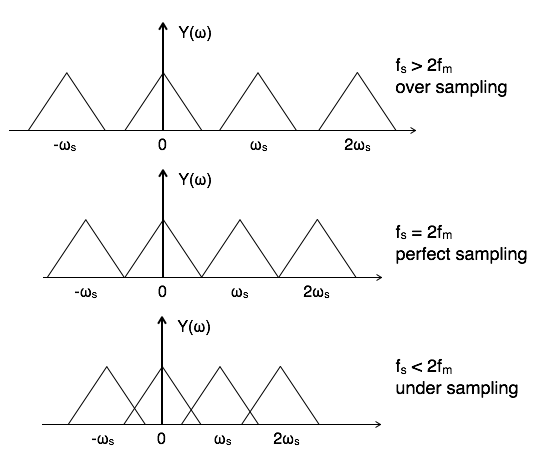
\includegraphics[width=0.7\textwidth]{./perfect_sampling.png}
	\caption{Casos do Sampling Theorem}
	\label{fig:aliasing}
\end{figure}

Este fenômeno pode ser evitado aplicando, previamente à amostragem, um filtro passa-baixa no sinal original, de forma que a banda do sinal seja reduzida, garantindo que \( \omega_s \geq 2\omega_c \), permitindo então a reconstrução do sinal.

% ==================================================================================
% ==================================================================================
% ==================================================================================
% ==================================================================================
% ==================================================================================
% ==================================================================================
% ==================================================================================

\section*{\textbf{Questão 5}}
\addcontentsline{toc}{section}{Questão 5}

\textit{Demostre a seguinte expressão da aula 4:}

\begin{equation*}
	v = \psi u
\end{equation*}
onde
\begin{equation*}
	\psi = F \otimes F
\end{equation*}

\textbf{Resolução:}

Seja $u(m,n)\in R^{N \times N}$ uma imagem e $v(k,l)\in R^{N \times N}$ sua respectiva DFT, onde a transformada de Fourier é definida como:

\begin{equation*}
	F=\{\dfrac{1}{\sqrt{N}}\exp(-2\pi j \dfrac{kn}{N}), 0 \leq k,n \leq N-1\}
\end{equation*}

Logo, o cálculo da transformada de $u(m,n)$ em duas dimensões é dada por:

\begin{equation*}
	v(k,l) = \dfrac{1}{N} \sum_{m = 0}^{N-1} \sum_{n = 0}^{N-1} \exp(-2\pi j \dfrac{km}{N}) u(m,n)\exp(-2\pi j \dfrac{ln}{N}).
\end{equation*}

Para simplificar a escrita, vamos adotar a seguinte notação:

\begin{equation*}
	F(p,q) = \dfrac{1}{\sqrt{N}}\exp(-2\pi j \dfrac{pq}{N})
\end{equation*}

Logo:

\begin{equation*}
	v(k,l) = \dfrac{1}{N} \sum_{m = 0}^{N-1} \sum_{n = 0}^{N-1} F(k,m) u(m,n)F(l,n).
\end{equation*}

Para representar $u$ e $v$ como vetores, considerando a indexação começando por $0$, teremos que:

\begin{equation*}
	u(m,n) = \vec{u}(m(N-1)+n)
\end{equation*}

onde

\begin{equation*}
	\vec{u} = \begin{pmatrix}
		\vec{u}(0\cdot N+0) = u(0,0) \\
		\vec{u}(0\cdot N+1) = u(0,1) \\
		\vdots \\
		\vec{u}(0\cdot N+(N-1)) = u(0,N-1) \\
		\vec{u}(1\cdot N + 0) = u(1,0) \\
		\vdots \\
		\vec{u}(1\cdot N+(N-1)) = u(1,N-1)\\
		\vdots \\
		\vec{u}((N-1)N + (N-1)) = u(N-1,N-1)
		\end{pmatrix}
\end{equation*}

logo, $\vec{u}, \vec{v} \in R^{N^2}$.

Então, vetorizando, a DFT ficaria então definida como:

\begin{equation*}
	\vec{v}(k\cdot N + l) = \sum_{m=0}^{N-1} \sum_{n=0}^{N-1} F(k,m) \cdot \vec{u}(m\cdot N + n) \cdot F(l,n)
\end{equation*}

Além disso, temos que o produto de Kronecker $F \otimes F \in R^{N^2 \times N^2}$ é dado por:

\begin{equation*}
	F \otimes F = \begin{pmatrix}
		F(0,0)\cdot F && \cdots && F(0,N-1)\cdot F \\
		\vdots && \ddots && \vdots  \\
		F(N-1,0)\cdot F && \cdots && F(N-1,N-1)\cdot F
		\end{pmatrix}
\end{equation*}

onde:

\begin{equation*}
	F(p,q) \cdot F = \begin{pmatrix}
		F(p,q)\cdot F(0, 0) && \cdots && F(p,q)\cdot F(0, N-1) \\
		\vdots && \ddots && \vdots  \\
		F(p,q)\cdot F(N-1,0) && \cdots && F(p,q)\cdot F(N-1,N-1)
		\end{pmatrix}
\end{equation*}

Observe que a $(k\cdot N+l)$-ésima linha de $F \otimes F$ é dada por:

\begin{equation*}
		F(k,0)\cdot F(l,0) \cdots F(k,0)\cdot F(l,N-1) \cdots F(k,N-1)\cdot F(l,0) \cdots F(k,N-1)\cdot F(l,N-1)
\end{equation*}

Logo, sabendo que múltiplicação entre $F \otimes F$ e $\vec{u}$ está bem definida já que $F \otimes F\in R^{N^2\times N^2}$ e $\vec{u}\in R^{N^2}$, teremos então que a multiplicação entre a $(k\cdot N+l)$-ésima linha de $F \otimes F$ e $\vec{u}$ resultará em:

\begin{equation*}
	F(k,0)\cdot F(l,0) \cdot \vec{u}(0\cdot N + 0) + \cdots +  F(k,0)\cdot F(l,N-1) \vec{u}(0\cdot N + (N-1)) + \cdots + 
\end{equation*}

\begin{equation*}
	F(k,N-1)\cdot F(l,N-1)\vec{u}((N-1)\cdot N + (N-1)) = \sum_{m=0}^{N-1} \sum_{n=0}^{N-1} F(k,m) \cdot F(l,n) \cdot \vec{u}(m\cdot N+n) = 
\end{equation*}

\begin{equation*}
	\sum_{m=0}^{N-1} \sum_{n=0}^{N-1} F(k,m) \cdot \vec{u}(m\cdot N+n) \cdot F(l,n) =  \vec{v}(k\cdot N + l)
\end{equation*}

Portanto, como vale para quaisquer $k,l \in \{0,1,\ldots, N-1\}$, podemos então concluir que:

\begin{tcolorbox}
\[
	\vec{v} = F\otimes F \cdot \vec{u}
\]
\end{tcolorbox}


\end{document}
